% fig07_zonal_geometry.tex
% Standalone TikZ: Zonal potential geometry — r, z-hat, u = omega + f
\documentclass[tikz,border=5pt]{standalone}
\usepackage{amsmath,amssymb}
\usetikzlibrary{arrows.meta,calc,decorations.pathreplacing,decorations.markings,
                positioning,3d,patterns}

\definecolor{accent}{RGB}{0, 100, 170}
\definecolor{highlight}{RGB}{200, 60, 30}
\definecolor{darkgreen}{RGB}{0, 120, 60}
\definecolor{earthblue}{RGB}{40,80,150}
\definecolor{orbitgray}{RGB}{100,100,100}

\begin{document}
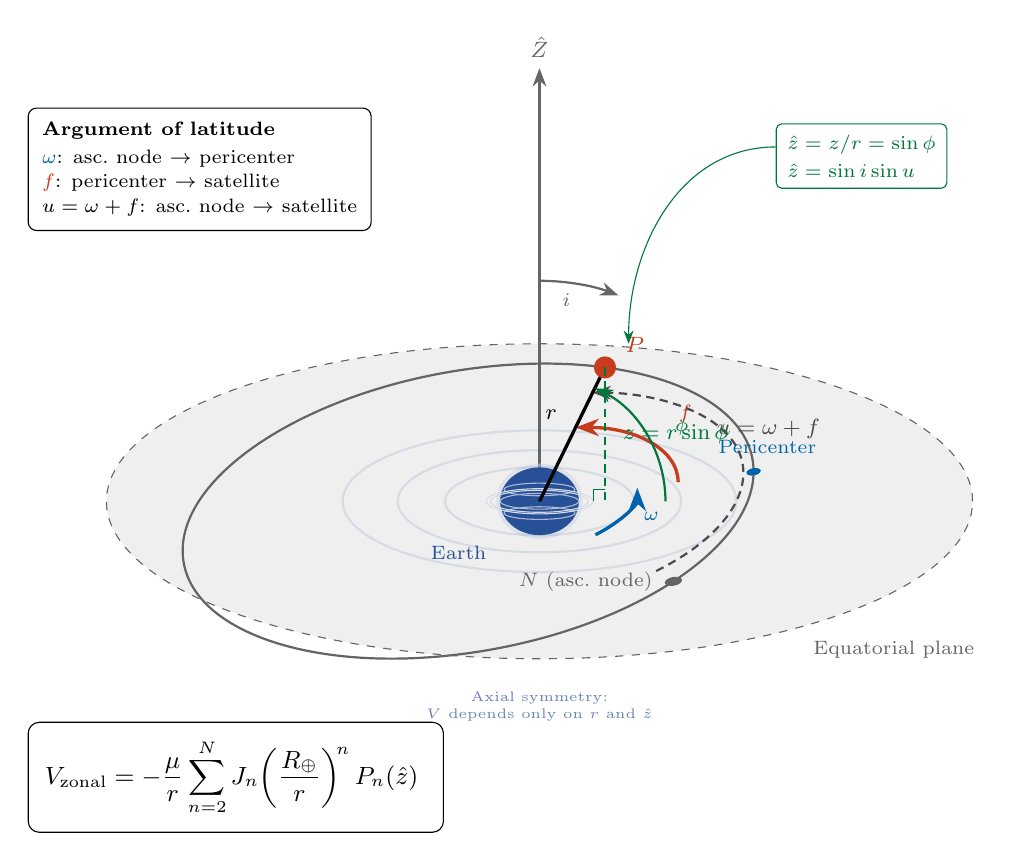
\begin{tikzpicture}[
    >=Stealth,
    font=\footnotesize,
    scale=1.0,
  ]

  %% ── Parameters (all defined at top level so they survive scopes) ──
  \pgfmathsetmacro{\inc}{50}
  \pgfmathsetmacro{\sma}{3.5}
  \pgfmathsetmacro{\ecc}{0.25}
  \pgfmathsetmacro{\smb}{\sma*sqrt(1-\ecc*\ecc)}
  \pgfmathsetmacro{\focalShift}{\sma*\ecc}
  \pgfmathsetmacro{\opXx}{1.0}   \pgfmathsetmacro{\opXy}{0.0}
  \pgfmathsetmacro{\opYx}{0.42*cos(\inc)}  \pgfmathsetmacro{\opYy}{sin(\inc)*0.72}
  \pgfmathsetmacro{\argNode}{15}
  \pgfmathsetmacro{\omegaArg}{55}
  \pgfmathsetmacro{\nodeTA}{360 - \omegaArg}
  \pgfmathsetmacro{\trueAnom}{75}
  \pgfmathsetmacro{\rsat}{\sma*(1-\ecc*\ecc)/(1+\ecc*cos(\trueAnom))}
  \pgfmathsetmacro{\rNodeVal}{\sma*(1-\ecc*\ecc)/(1+\ecc*cos(\nodeTA))}
  % Screen-space satellite position
  \pgfmathsetmacro{\satScreenTA}{\trueAnom + \argNode}
  \pgfmathsetmacro{\satSx}{\rsat*(\opXx*cos(\satScreenTA) + \opYx*sin(\satScreenTA))}
  \pgfmathsetmacro{\satSy}{\rsat*(\opXy*cos(\satScreenTA) + \opYy*sin(\satScreenTA))}
  % Screen-space node position
  \pgfmathsetmacro{\nodeScreenTA}{\nodeTA + \argNode}
  \pgfmathsetmacro{\nodeSx}{\rNodeVal*(\opXx*cos(\nodeScreenTA) + \opYx*sin(\nodeScreenTA))}
  \pgfmathsetmacro{\nodeSy}{\rNodeVal*(\opXy*cos(\nodeScreenTA) + \opYy*sin(\nodeScreenTA))}
  % Phi angle for labeling
  \pgfmathsetmacro{\satAngleScreen}{atan2(\satSy, \satSx)}

  %% ── Equatorial plane (light gray disk) ──
  \begin{scope}[opacity=0.10]
    \fill[orbitgray] (0,0) ellipse (5.5cm and 2.0cm);
  \end{scope}
  \draw[orbitgray, thin, dashed] (0,0) ellipse (5.5cm and 2.0cm);
  \node[orbitgray, anchor=north] at (4.5, -1.65) {\scriptsize Equatorial plane};

  %% ── Z axis ──
  \draw[->, thick, black!60] (0,0) -- (0, 5.5) node[above] {$\hat{Z}$};

  %% ── Earth (oblate, with zonal symmetry cue) ──
  \begin{scope}
    \fill[earthblue!25, opacity=0.5] (0,0) ellipse (0.55cm and 0.48cm);
    \fill[earthblue] (0,0) ellipse (0.50cm and 0.43cm);
    % Latitude lines to suggest zonal symmetry
    \draw[earthblue!40, thin] (0, 0.15) ellipse (0.45cm and 0.08cm);
    \draw[earthblue!40, thin] (0,-0.15) ellipse (0.45cm and 0.08cm);
    \draw[earthblue!40, thin] (0, 0) ellipse (0.50cm and 0.10cm);
    % Equatorial bulge hint (faint outer ring)
    \draw[earthblue!20, thin] (0,0) ellipse (0.62cm and 0.14cm);
    \draw[earthblue!20, thin] (0,0) ellipse (0.68cm and 0.16cm);
  \end{scope}
  \node[earthblue, anchor=north east, font=\scriptsize] at (-0.55, -0.45)
    {Earth};

  %% ── Orbital plane and orbit ellipse ──
  \begin{scope}[
    cm={\opXx,\opXy,\opYx,\opYy,(0,0)},
    rotate=\argNode,
  ]
    %% ── Orbit ellipse ──
    \draw[orbitgray, thick] (-\focalShift, 0) ellipse ({\sma} and {\smb});

    %% ── Ascending node ──
    \coordinate (Node) at ({\rNodeVal*cos(\nodeTA)}, {\rNodeVal*sin(\nodeTA)});
    \fill[orbitgray] (Node) circle (3pt);

    %% ── Pericenter ──
    \coordinate (Peri) at ({-\focalShift + \sma}, 0);
    \fill[accent] (Peri) circle (2.5pt);
    \node[accent, anchor=south, yshift=3pt, xshift=5pt, font=\scriptsize]
      at (Peri) {Pericenter};

    %% ── Satellite position ──
    \coordinate (SatOrb) at ({\rsat*cos(\trueAnom)}, {\rsat*sin(\trueAnom)});

    %% ── omega arc: from ascending node to pericenter ──
    \pgfmathsetmacro{\arcRom}{1.2}
    \draw[accent, very thick, ->]
      ({\arcRom*cos(\nodeTA)}, {\arcRom*sin(\nodeTA)})
      arc[start angle=\nodeTA, end angle=360, radius=\arcRom];
    \node[accent, font=\scriptsize] at
      ({1.55*cos(\nodeTA + 0.5*\omegaArg)}, {1.55*sin(\nodeTA + 0.5*\omegaArg)})
      {$\omega$};

    %% ── f arc: from pericenter to satellite ──
    \pgfmathsetmacro{\arcRf}{1.7}
    \draw[highlight, very thick, ->]
      (\arcRf, 0) arc[start angle=0, end angle=\trueAnom, radius=\arcRf];
    \node[highlight, font=\scriptsize, anchor=south west] at
      ({2.0*cos(0.5*\trueAnom)}, {2.0*sin(0.5*\trueAnom)})
      {$f$};

    %% ── u = omega + f combined arc ──
    \pgfmathsetmacro{\arcRu}{2.5}
    \pgfmathsetmacro{\uTotal}{360 - \nodeTA + \trueAnom}
    \draw[black!70, thick, densely dashed, ->]
      ({\arcRu*cos(\nodeTA)}, {\arcRu*sin(\nodeTA)})
      arc[start angle=\nodeTA, end angle={\nodeTA + \uTotal}, radius=\arcRu];
    \node[black!70, font=\footnotesize, anchor=south] at
      ({2.85*cos(\nodeTA + 0.5*\uTotal)}, {2.85*sin(\nodeTA + 0.5*\uTotal)})
      {$u = \omega + f$};

    %% ── r line from Earth center to satellite ──
    \draw[black, very thick] (0,0) -- (SatOrb);
  \end{scope}

  %% ── Satellite dot (in screen coordinates, on top) ──
  \fill[highlight] (\satSx, \satSy) circle (4pt);
  \node[highlight, anchor=south west, xshift=4pt, yshift=2pt]
    at (\satSx, \satSy) {$P$};

  %% ── r label ──
  \node[black, anchor=south east, font=\footnotesize, xshift=-2pt, yshift=2pt]
    at ({0.5*\satSx}, {0.5*\satSy}) {$r$};

  %% ── Ascending node label ──
  \node[orbitgray, anchor=east, xshift=-4pt, font=\scriptsize]
    at (\nodeSx, \nodeSy) {$N$ (asc.\ node)};

  %% ── Vertical line from satellite to equatorial plane (z component) ──
  \draw[darkgreen, densely dashed, thick]
    (\satSx, \satSy) -- (\satSx, 0);
  % Small right-angle mark
  \draw[darkgreen, thin]
    ({\satSx - 0.15}, 0.0) -- ({\satSx - 0.15}, 0.15) -- (\satSx, 0.15);
  % z label
  \node[darkgreen, anchor=west, xshift=3pt, font=\footnotesize]
    at (\satSx, {0.5*\satSy}) {$z = r\sin\phi$};

  %% ── phi (geocentric latitude) arc ──
  \pgfmathsetmacro{\phiArcR}{1.6}
  \draw[darkgreen, thick, ->]
    (\phiArcR, 0) arc[start angle=0, end angle=\satAngleScreen, radius=\phiArcR];
  \node[darkgreen, font=\scriptsize, anchor=west, xshift=2pt]
    at ({1.8*cos(0.5*\satAngleScreen)}, {1.8*sin(0.5*\satAngleScreen)}) {$\phi$};

  %% ── z-hat relation annotation ──
  \node[darkgreen, anchor=north west, font=\scriptsize, align=left,
        draw, rounded corners=2pt, fill=white, fill opacity=0.9, text opacity=1,
        inner sep=4pt]
    at (3.0, 4.8) {%
    $\hat{z} = z/r = \sin\phi$\\[2pt]
    $\hat{z} = \sin i \sin u$
  };
  \draw[->, darkgreen, thin] (3.0, 4.5) to[out=180, in=90]
    ({\satSx + 0.3}, {\satSy + 0.3});

  %% ── Inclination angle ──
  \draw[black!60, thick, ->]
    (0, 2.8) arc[start angle=90, end angle={90 - \inc*0.42}, radius=2.8cm];
  \node[black!60, font=\scriptsize, anchor=east, xshift=-1pt]
    at (0.55, 2.55) {$i$};

  %% ── Zonal symmetry annotation (concentric bulge arcs) ──
  \begin{scope}[opacity=0.12]
    \foreach \rr in {1.2, 1.8, 2.5} {
      \draw[earthblue, thick] (0,0) ellipse ({\rr cm} and {\rr*0.36 cm});
    }
  \end{scope}
  \node[earthblue!70, anchor=north, font=\tiny, align=center] at (0, -2.3)
    {Axial symmetry:\\$V$ depends only on $r$ and $\hat{z}$};

  %% ── Formula box ──
  \node[draw, rounded corners=4pt, fill=white, fill opacity=0.95, text opacity=1,
        inner sep=6pt, anchor=north west, font=\small,
        align=left] at (-6.5, -2.8) {%
    $\displaystyle V_{\text{zonal}} =
      -\frac{\mu}{r}\sum_{n=2}^{N} J_n
      \!\left(\frac{R_\oplus}{r}\right)^{\!n}
      P_n(\hat{z})$
  };

  %% ── Argument of latitude annotation ──
  \node[draw, rounded corners=3pt, fill=white, fill opacity=0.92, text opacity=1,
        inner sep=5pt, anchor=north west, font=\scriptsize,
        align=left] at (-6.5, 5.0) {%
    \textbf{Argument of latitude}\\[2pt]
    \textcolor{accent}{$\omega$}: asc.\ node $\to$ pericenter\\[1pt]
    \textcolor{highlight}{$f$}: pericenter $\to$ satellite\\[1pt]
    $u = \omega + f$: asc.\ node $\to$ satellite
  };

\end{tikzpicture}
\end{document}
